\documentclass[12pt,a4]{article}
\usepackage[utf8]{inputenc}
\usepackage{natbib}
\usepackage[a4paper,left=2.5cm,right=2.5cm,top=2.5cm,bottom=2.5cm]{geometry}

\usepackage{multicol,caption}
\usepackage{graphicx}
\usepackage{wrapfig}
\usepackage{tabto}
\usepackage{float}
\usepackage{subfig}
\usepackage{amsfonts}
\usepackage{amsmath}
\usepackage{ragged2e}
\usepackage{amsmath}
\usepackage{hyperref}
\usepackage{parskip}
\usepackage[table,xcdraw]{xcolor}

\setlength{\parskip}{12pt}
\setlength{\parindent}{15pt}

\begin{document}
\vspace*{\fill}
    \begin{center}
    
        \huge{\textbf{INF552 - Data Visualization}}
        \huge{\textbf{Brazilian Export Historical Data}}
        
        
        \vspace{3cm}
        \normalsize
        
        Abdoul Rahim\\
        Guilherme Vieira\\
 
        \vspace{1cm}
        
        11 December, 2023
       
    \end{center}

\vspace*{\fill}


\newpage

\section{Introduction}
With this project we wanted to apply the concepts we learned throughout the course and the techniques learned in TD to create a clean, interactive and complete visualization of Brazilian export historical data. In this report we explain in detail what was the rationale behind the dataset choice, the technical challenges we faced during development and the design choices we have made for our visualizations. 

The project code can be found on \href{http://www.github.com/guilevieiram/BRViz}{GitHub}. There you  will find instructions on how to download, install and run the application locally. Along with this report you will find a gallery and a video demo of the application.

To view a live version of the project please visit \href{http://18.170.60.53}{http://18.170.60.53}. Since this is only a demo version, the website can be unstable and only an http version is available.

\section{Dataset}
As presented on the abstract of the dataset on kaggle, our dataset is generated by the \textbf{Brazilian Federal Government} and finely presents all the data used to construct the Brazilian trade balance from 1996 to 2023. It is made up of a total of 26921053 rows with 11 columns. But for the time of computational calculations, we only use 1\% of the dataset and 5 of the columns, listed below.: 

\begin{itemize}
    \item CO\_ANO : the year of data disclosure
    \item CO\_MES : the months code (1:January 12:December)
    \item CO\_NCM : the \href{https://www.novatradebrasil.com/en/customs-code-classification-brazil-ncm/}{Mercosul Common Nomenclature} code of the merchandise
    \item CO\_VIA: the code to identify the means of transport used (air, sea, road, rail, and others)
    \item KG\_NET: the measure that expresses the net weight of the merchandise. Even products whose statistical quantities are not kilograms also have a measurement in kilograms, which corresponds to the net weight of the goods
\end{itemize}
Through the visualization we've made using the datasets, we're trying to show certain known facts, such as the most exported products from Brazil being mineral products. We also try to see the dynamics in the countries that represent Brazil's main trading partners, and in these exchanges, which means of transport are most used, are they linked to the distance between the two countries, etc.... Finally, we intended to identify the effects of the formation of trading blocs on Brazil exports.

\section{Technical challanges}

To be able to properly visualize our dataset, many technical decisions and adaptations have been made to ensure performance, a good user experience and ease-of-development.

\subsection{Performance}

In terms of performance, we have opted to separate our application in two parts: a client (frontend) and a server (backend). While the client takes care of mounting the graphics and the interactivity, the server specializes in heavy data processing and serving that data over an API. This choice allowed us to have a performant compiled language serving already processed data via an API and reduce the amount of computations done in the client browser (Javascript). The necessity for this architectural choice came mainly from the volume of the data in hand: over 26 million lines of data spanning many columns. Early tests revealed that it was impossible to process even 0.1\% of that directly in the browser. 

The technology chosen to create this server was Golang: a compiled statically typed language that has an easy to use interface and is specialized in creating web API’s. The server setup was fairly easy using the standard library. However, reading and processing the data was harder since no out-of-the box solutions are available. For that we have developed our own data processing module with capabilities to batch-read CSV files, filter data by column values, aggregate data on a column and serve a subset of the data. Integrating this library on our API allowed for an easy client interface where the Javascript can specify exactly which columns, which rows, aggregated by what, it needs. 

Even with the highly performant server in hands, the dataset was too large to be loaded at once in memory, consuming over 8GB of RAM. To surpass this issue we have downsized the dataset to 1\% of its original size via random sampling. We estimate that using an actual server with more memory capacity could make possible the visualization of the whole dataset by a client, however this falls out of the project scope. 

\subsection{User Experience}
Our plan to visualize this dataset was to provide a large set of interactive visualizations for the user to explore the data and gain insights on the Brazilian exports. To make this accessible from different devices, we have decided to make a Web Application. This app would make possible the implementation of a clean and intuitive user interface powered by a routing system.

\subsection{Ease of Development}
Since the members of the group had a certain familiarity with web development, and specially the React framework, we have decided to use it for the client. The reactivity desired in the visualizations and the routing system have also empowered this choice. For the website styling we relied on a framework called TailwindCSS and also raw CSS in some cases. To help develop all the visualizations we envisioned, we made use of another framework \href{https://nivo.rocks/}{Nivo}. This library is a wrapper around d3 that creates powerful and easy to use components for many different visualizations. This library has yielded high quality graphics that can be extended using all the d3 functionalities seen in the course.

In the end, the stack and technologies we chose allowed us to surpass technical difficulties while still maintaining ease of development to focus on the important part: the visualizations and the user experience/exploration.


\section{Design}

The visualizations provided in this application were crafted by considering the data format we had in hand, which kinds of data we could easily access and the insights we wanted to explore. 

Categorical features such as means of transportation and product category were not well described in the original dataset but were widely available in official government websites. Other quantitative features, such as weight, were key to separate countries and measure proportions in the exports.

Here we provide an overview of the different visualizations developed as well as the features they explore and their interactivity.

\subsection{Area Bump}

We provide two different Area Bump maps in the application both plotting a categorical feature over time (on the x axis) and by weight (thickness of the line). The first graph explores the product categories (Category Stratification Over Time) whereas the second one explores the partner countries in trading (Countries Commerce Over time).

We have chosen to use an Area Bump over a simple line plot (for example) for a couple of reasons. Firstly the proportions of export among different categories and countries would make it hard to distinguish between different countries / categories. Secondly, with an Area Bump we have the ranking information (who was ranked first, second, etc) in that feature. Thirdly, we still have the weight information being visualized over time for each country/category separately, which can bring many insights. For example we see that Mining had a great increase in exports around 2015, which is mostly due to the discovery of new mines by Vale, a colossal mining company. Also, we can see a boom in Chinese relations after the consolidation of the BRICS economic block in 2011 that brought the two countries closer.

In the categories graph we take advantage of the arborescent structure of the classification to provide yet another stratification. Upon clicking on the band for a category, for example Ores, Slag and Ash, you are presented with all its subcategories, most predominantly Iron Ore. This provides another layer of exploration within the NCM product classification scheme.

It is worth noting that we only considered the top 10 for those graphs and used a categorical color scheme to better distinguish values.

\begin{figure}[H]
    \centering
    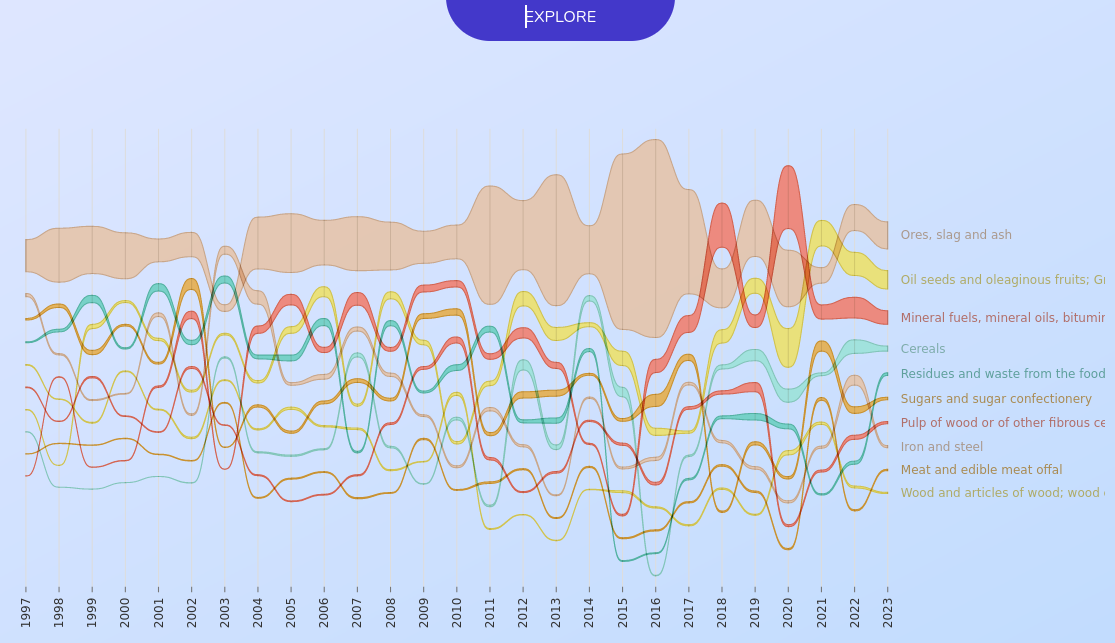
\includegraphics[width=0.9\textwidth]{assets/bump1.png}
    \caption{Area Bump of main categories over time}
\end{figure}

\begin{figure}[H]
    \centering
    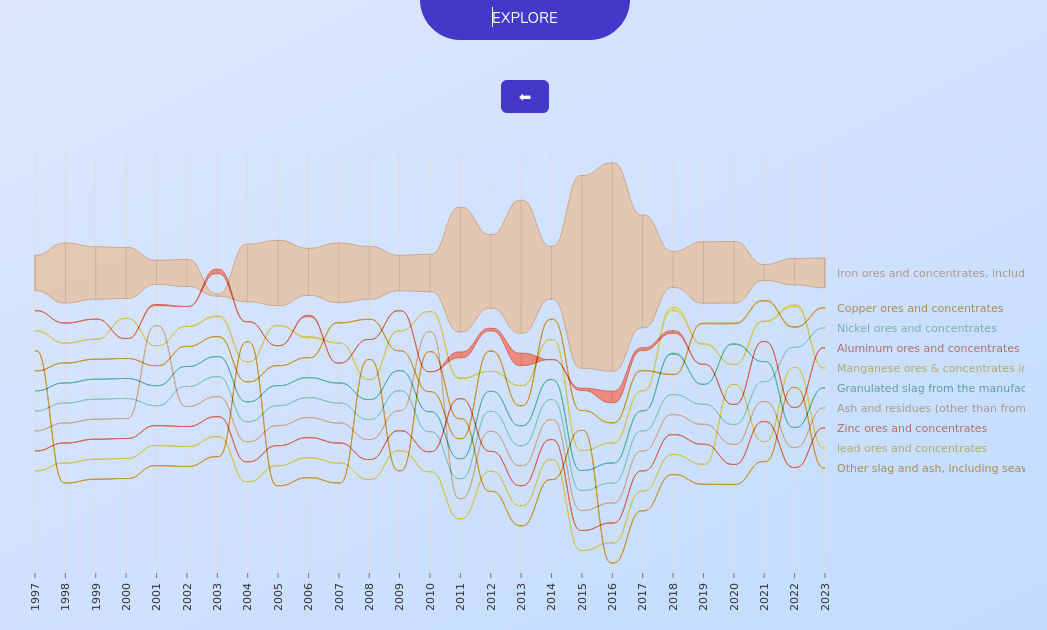
\includegraphics[width=0.9\textwidth]{assets/bump2.png}
    \caption{Area Bump of categories under Ore, Slag and Ash over time}
\end{figure}

\begin{figure}[H]
    \centering
    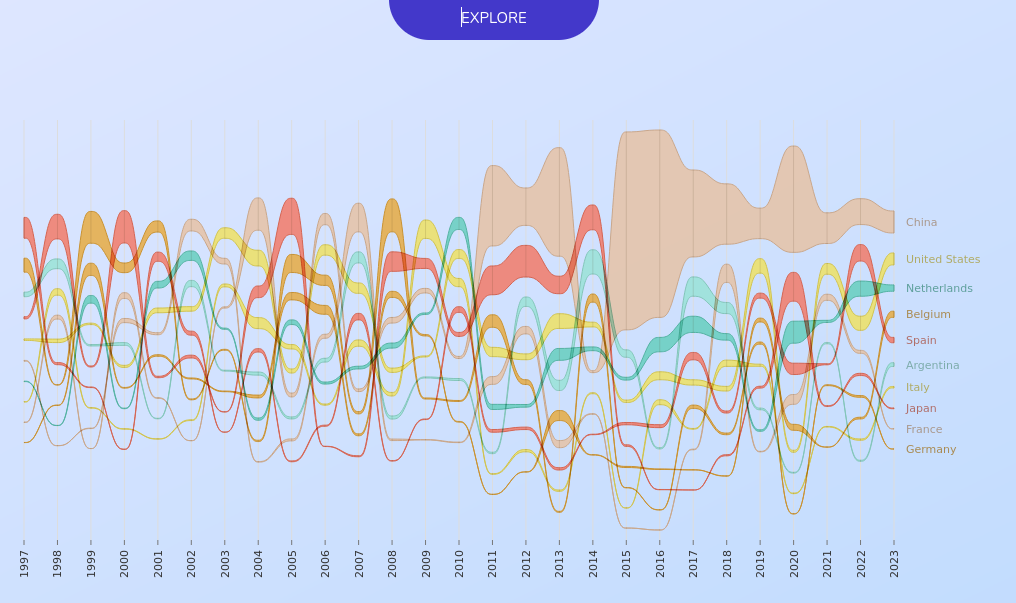
\includegraphics[width=0.9\textwidth]{assets/countries1.png}
    \caption{Area Bump of Countries over time}
\end{figure}

\subsection{Stream}
The “Weight over Time Stratified By Country” allows you to select on a globe map any country and from there visualize the 5 most traded category of products for each year. For this exploration we used a Stream graph since it clearly shows the proportions between the categories over time. To better distinguish the data we included a hover that shows for each year the values (in Kg) of the total trade and the name of the categories. 

This visualization was constructed with the intent of seeing how the exports profile of Brazil changed with respect to each country over time. For example, the USA lowered their Iron import from 2015 to 2021 and prioritized the import of mineral fuels.

\begin{figure}[H]
    \centering
    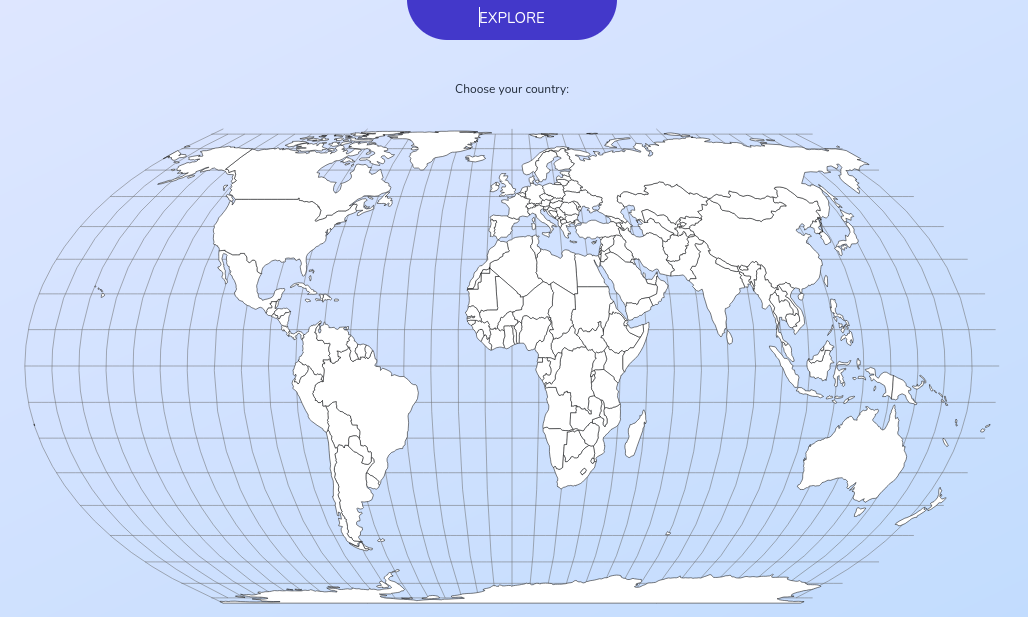
\includegraphics[width=0.9\textwidth]{assets/stream1.png}
    \caption{Selecition map}
\end{figure}

\begin{figure}[H]
    \centering
    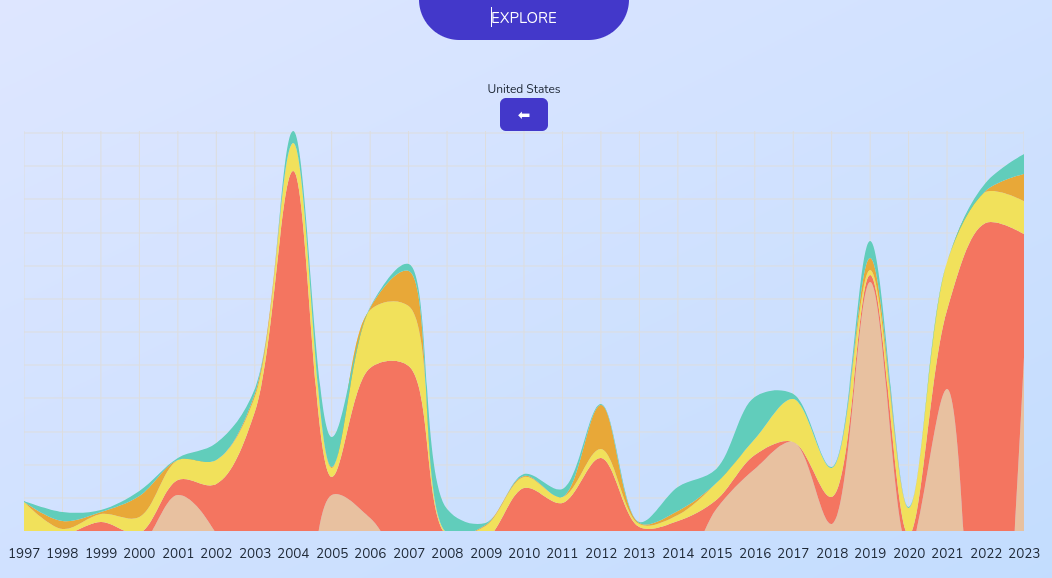
\includegraphics[width=0.9\textwidth]{assets/stream2.png}
    \caption{Stream of weight over time for the USA}
\end{figure}

\subsection{Heatmaps}
Heatmaps are a great way of viewing the correlation between two categorical variables on a quantitative feature. We have used them to plot the total weight (summed over all available years) of product against country and of transportation mean against country. To better distinguish the different orders of magnitude of trade we used a log color scale in blue tones to color the cells in the matrix.

We have also added a layer of interactivity that, on hover, highlights the corresponding row and column, allowing for easy comparisons of a feature (category or transportation) inside a country or comparison between countries.

In these visualizations we have only considered the 10 most traded categories and countries. We have considered all the means of transportation, even though many of them have a very low count.

There are some nice insights to take from these heatmaps. For example, Japan is the second most Ores importer, consuming over 5 times the US amount. Also, China is by far the largest consumer of oil seeds and grains (probably Soya).  In means of transport we see that the scenario is dominated by Maritime transport because of global trade. We also notice that neighboring countries like Argentina tend to receive a lot of products via Highway.

\begin{figure}[H]
    \centering
    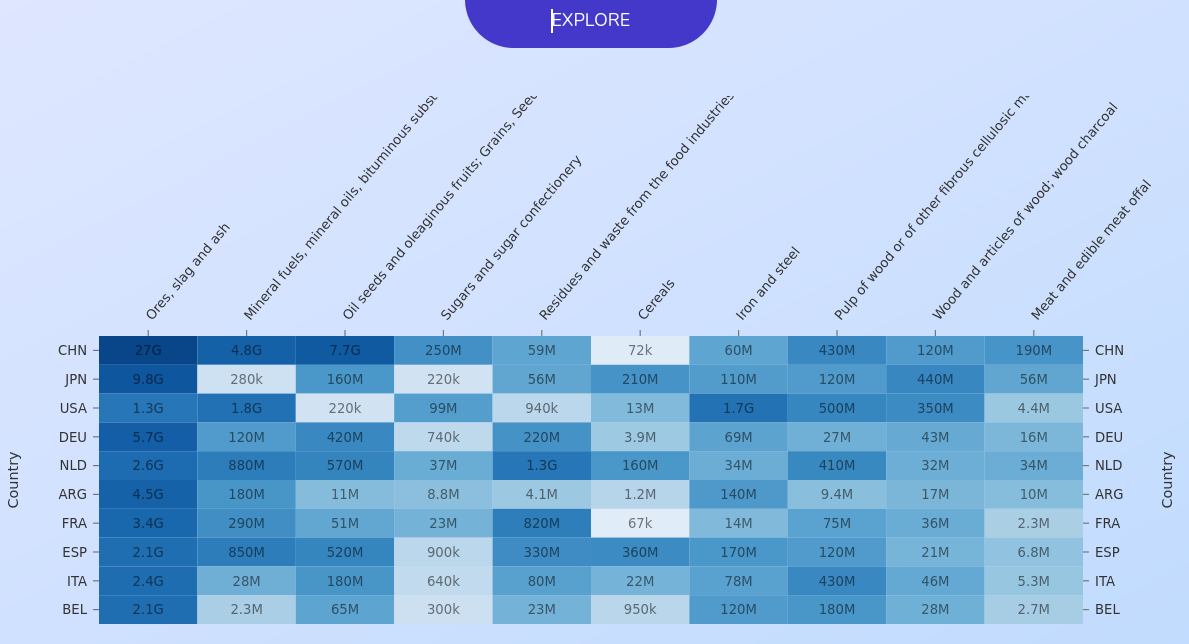
\includegraphics[width=0.9\textwidth]{assets/heat1.png}
    \caption{Categories vs Countries heatmap}
\end{figure}

\begin{figure}[H]
    \centering
    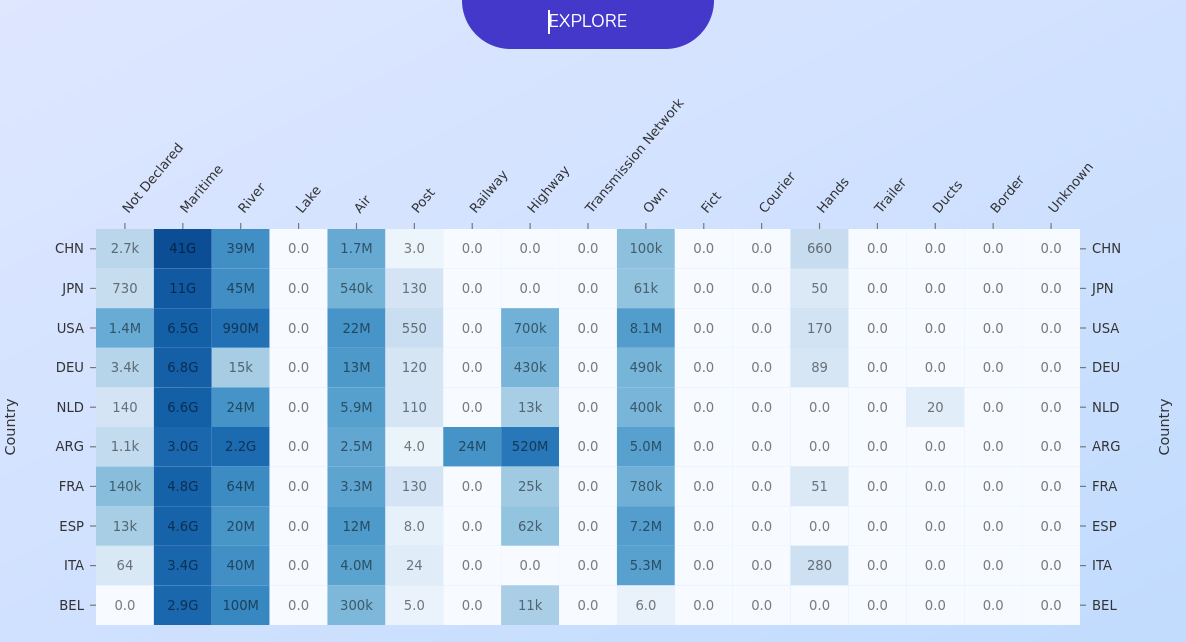
\includegraphics[width=0.9\textwidth]{assets/heat2.png}
    \caption{Means of transportation vs Countries heatmap}
\end{figure}

\subsection{Bar plot}
Another visualization we wanted to explore is how countries compare in total trade weight over different categories. For this we made use of a Bar plot of total product weight by country. We have stratified this on the y-axis by stacking different product categories. This allows us to see the trade proportions of different categories for each country and also to compare countries in both total trade size and inside each category.

For an extra interactivity component, we included a filter that allows you to remove/reinsert a given category by clicking on the corresponding legend. This allows us to really focus on the products we want to analyze at a given time. It is also a nice feature to have given the disproportional amount certain categories (like Ore) are traded, that hide all the other information from the graph.


\begin{figure}[H]
    \centering
    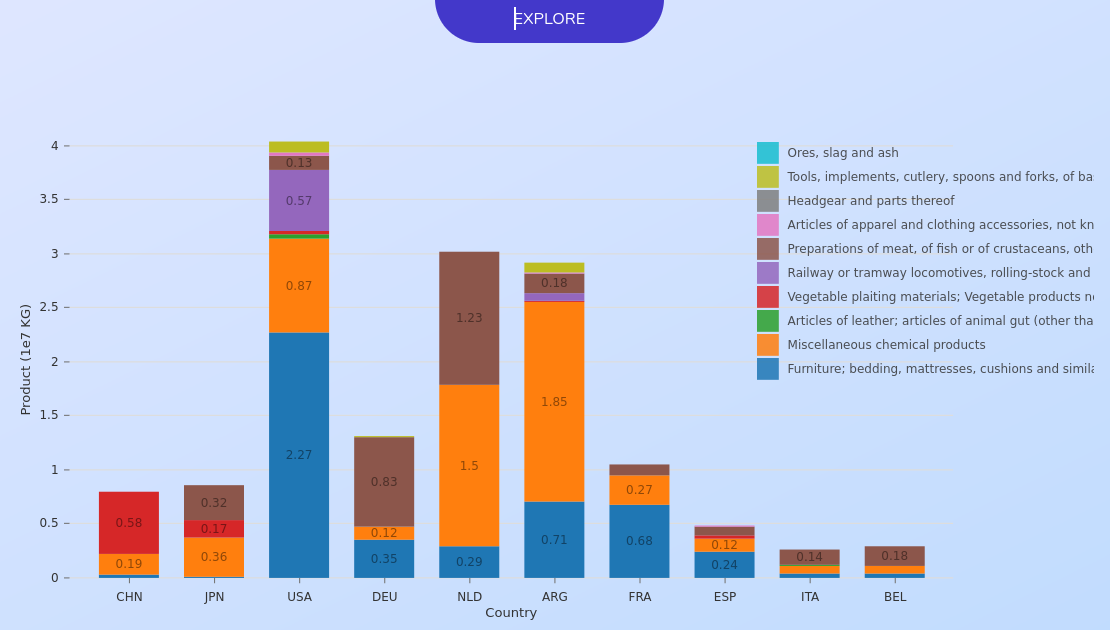
\includegraphics[width=0.9\textwidth]{assets/bar2.png}
    \caption{Barplot of weight by country satratified by category.}
\end{figure}

\subsection{Sunburst}
We try to use a sunburst chart to show the composition of the 10 largest product categories exported in a given year between 1996 and 2023. Since the sunburst chart is ideal for displaying hierarchical data and that product categories are hierarchical data (a tree such 
that the further down you go, the more polished the products), we thought this was a judicious choice.

We have a year slider at the bottom of the graph, which allows you to click on the year to see the corresponding distribution of the major categories for that year. For greater interactivity, we've added a tooltip displaying the categories' nomenclature and the quantity of their products. In addition, it is possible to click on each major category to obtain a more detailed breakdown of sub-categories. This feature offers a dynamic and comprehensive view, enabling users to explore and analyze data in depth, highlighting significant trends and insights in a user-friendly and visually appealing way.

\begin{figure}[H]
    \centering
    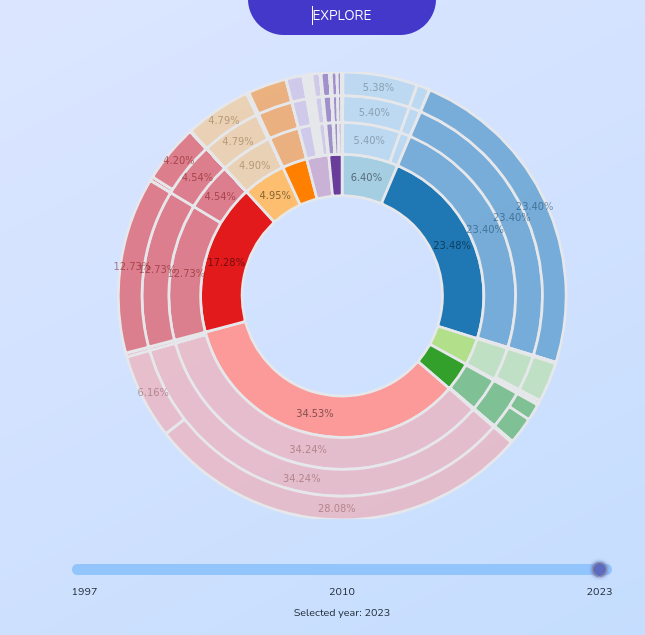
\includegraphics[width=0.9\textwidth]{assets/sun1.png}
    \caption{Categories Sunburst for 2023}
\end{figure}

\subsection{Swarm plot}
Like the sunburst chart, the swarm chart features a year slider at the bottom. It displays the means of transport used to deliver the different product categories, highlighting the total quantity of products in those categories at a selected year.

The use of the swarm diagram is justified by its ability to categorize and present data efficiently, which is particularly useful for analyzing transport trends over time.

Based on the graphs obtained, it can be seen that over the years the most substantial products have been transported by sea.

\begin{figure}[H]
    \centering
    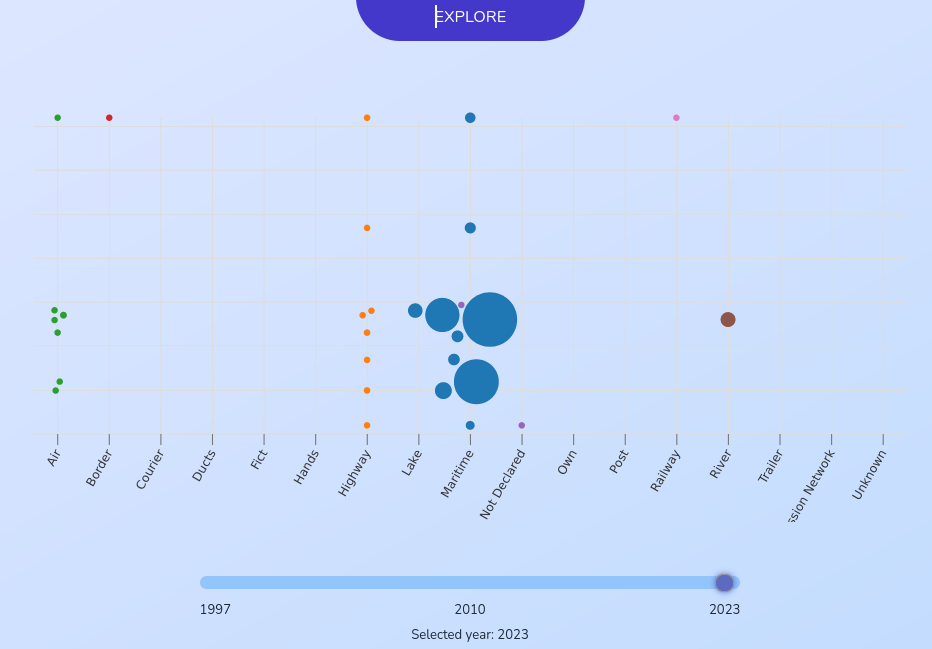
\includegraphics[width=0.9\textwidth]{assets/swarm1.png}
    \caption{Swarm plot for means of transportation at 2014}
\end{figure}
\subsection{Choropleth Map}
The last chart we made was a choropleth map with an option to select the year of the data to be displayed. The choropleth map shows the quantity of products imported by each country from Brazil. We also, thanks to a custom tooltip, added a list of the top 5 products imported by each country.

It gives you an overview of trade between Brazil and the rest of the world. In fact, we can see that Brazil doesn't export much to Central African countries, although there has been an increase in trade between Brazil and South Africa and India since the formation of the BRICS in 2011.

\begin{figure}[H]
    \centering
    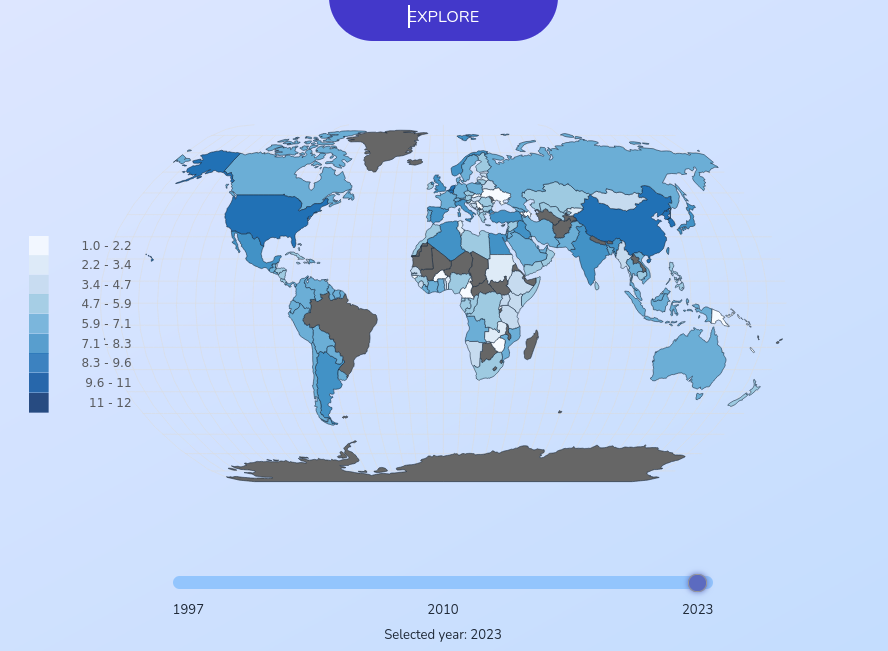
\includegraphics[width=0.9\textwidth]{assets/choro1.png}
    \caption{Choropleth Map for total export weight at 2023}
\end{figure}

\section{Conclusion}
In the end, we were able to develop a performant application that allows the user to explore interactively historical data on Brazil exports. This has been accomplished by applying the design concepts seen in the course together with the technical knowledge acquired during the TDs and during the development.

\end{document}
